
%(BEGIN_QUESTION)
% Copyright 2015, Tony R. Kuphaldt, released under the Creative Commons Attribution License (v 1.0)
% This means you may do almost anything with this work of mine, so long as you give me proper credit

\noindent
{\bf Lab Exercise -- introduction}

\vskip 5pt

Your task is to build, document, and troubleshoot a pressure measurement system consisting of an electronic $\Delta$P or gauge pressure transmitter connected to an electronic indicator, recorder, or indicating controller.  Instrument air pressure, either regulated or unregulated, is the suggested process variable to measure.  Other process variables are open for consideration, though.  Alternatives to the standard pressure-measurement lab are authorized by instructor permission only.

The following table of objectives show what you and your team must complete within the scheduled time for this lab exercise.  Note how some of these objectives are individual, while others are for the team as a whole:

\underbar{Objective completion table:}

% No blank lines allowed between lines of an \halign structure!
% I use comments (%) instead, so that TeX doesn't choke.

$$\vbox{\offinterlineskip
\halign{\strut
\vrule \quad\hfil # \ \hfil & 
\vrule \quad\hfil # \ \hfil & 
\vrule \quad\hfil # \ \hfil & 
\vrule \quad\hfil # \ \hfil & 
\vrule \quad\hfil # \ \hfil & 
\vrule \quad\hfil # \ \hfil & 
\vrule \quad\hfil # \ \hfil \vrule \cr
\noalign{\hrule}
%
% First row
{\bf Performance objective} & {\bf Grading} & {\bf 1} & {\bf 2} & {\bf 3} & {\bf 4} & {\bf Team} \cr
%
\noalign{\hrule}
%
% Another row
Team meeting and prototype sketch (do {\it first!}) & mastery & -- & -- & -- & -- & \cr
%
\noalign{\hrule}
%
% Another row
Circuit design challenge & mastery & & & & & -- -- -- -- \cr
%
\noalign{\hrule}
%
% Another row
Final loop diagram and system inspection & mastery & & & & & -- -- -- -- \cr
%
\noalign{\hrule}
%
% Another row
Digital trim (sensor and output) & mastery & -- & -- & -- & -- &  \cr
%
\noalign{\hrule}
%
% Another row
Loop ranging ($\pm$ 1\% of span accuracy) & mastery & & & & & -- -- -- -- \cr
%
\noalign{\hrule}
%
% Another row
Deadweight tester research and usage & mastery & & & & & -- -- -- -- \cr
%
\noalign{\hrule}
%
% Another row
Transmitter valve manifold usage & mastery & & & & & -- -- -- -- \cr
%
\noalign{\hrule}
%
% Another row
Troubleshooting & mastery & & & & & -- -- -- -- \cr
%
\noalign{\hrule}
%
% Another row
Lab question: Instrument connections & proportional &  &  &  &  & -- -- -- -- \cr
%
\noalign{\hrule}
%
% Another row
Lab question: Commissioning & proportional &  &  &  &  & -- -- -- -- \cr
%
\noalign{\hrule}
%
% Another row
Lab question: Mental math & proportional &  &  &  &  & -- -- -- -- \cr
%
\noalign{\hrule}
%
% Another row
Lab question: Diagnostics & proportional &  &  &  &  & -- -- -- -- \cr
%
\noalign{\hrule}
%
% Another row
Decommission and lab clean-up & mastery & -- & -- & -- & -- &  \cr
%
\noalign{\hrule}
} % End of \halign 
}$$ % End of \vbox

The only ``proportional'' scoring in this activity are the lab questions, which are answered by each student individually.  A listing of potential lab questions are shown at the end of this worksheet question.  The lab questions are intended to guide your labwork as much as they are intended to measure your comprehension, and as such the instructor may ask these questions of your team day by day, rather than all at once (on a single day).

\vskip 10pt

{\bf It is essential that your team plans ahead what to accomplish each day.  A short (10 minute) team meeting at the beginning of each lab session is a good way to do this, reviewing what's already been done, what's left to do, and what assessments you should be ready for.  There is a lot of work involved with building, documenting, and troubleshooting these working instrument systems!}

As you and your team work on this system, you will invariably encounter problems.  You should always attempt to solve these problems as a team before requesting instructor assistance.  If you still require instructor assistance, write your team's color on the lab whiteboard with a brief description of what you need help on.  The instructor will meet with each team in order they appear on the whiteboard to address these problems.

$$\includegraphics[width=15.5cm]{i00112x01.eps}$$





\vfil \eject

\noindent
{\bf Lab Exercise -- team meeting, prototype sketch, and instrument selection}

\vskip 5pt

An important first step in completing this lab exercise is to {\bf meet with your instructor} as a team to discuss safety concerns, team performance, and specific roles for team members.  If you would like to emphasize exposure to certain equipment (e.g. use a particular type of control system, certain power tools), techniques (e.g. fabrication), or tasks to improve your skill set, this is the time to make requests of your team so that your learning during this project will be maximized.

\vskip 10pt

An absolutely essential step in completing this lab exercise is to work together as a team to {\bf sketch a prototype diagram} showing what you intend to build.  This usually takes the form of a simple electrical schematic and/or loop diagram showing all electrical connections between components, as well as any tubing or piping for fluids.  This prototype sketch need not be exhaustive in detail, but it does need to show enough detail for the instructor to determine if all components will be correctly connected for their safe function.

For example, if you intend to connect field devices to a PLC (Programmable Logic Controller), your prototype sketch must show how those devices will connect to typical input/output terminals on the PLC, where electrical power will be supplied, etc.  Prototype sketches need not show all intermediary connections between components, such as terminal blocks in junction boxes between the field device and the controller.

You should practice good problem-solving techniques when creating your prototype sketch, such as consulting equipment manuals for information on component functions and marking directions of electric current, voltage polarities, and identifying electrical sources/loads.  Use this task as an opportunity to strengthen your analytical skills!  Remember that you will be challenged in this program to do all of this on your own (during ``capstone'' assessments), so do not make the mistake of relying on your teammates to figure this out for you -- instead, treat this as a problem {\it you} must solve and compare your results with those of your teammates.

Your team's prototype sketch is so important that the instructor will demand you provide this plan before any construction on your team's working system begins.  {\it Any team found constructing their system without a verified plan will be ordered to cease construction and not resume until a prototype plan has been drafted and approved!}  Similarly, you should not deviate from the prototype design without instructor approval, to ensure nothing will be done to harm equipment by way of incorrect connections.  Each member on the team should have ready access to this plan (ideally possessing their own copy of the plan) throughout the construction process.  Prototype design sketching is a skill and a habit you should cultivate in school and take with you in your new career.

\vskip 10pt

When selecting field instruments for this lab exercise, choose a {\it pressure transmitter} with electronic (4-20 mA) signal output as well as a valve ``manifold'' to isolate that transmitter from the process pressure.  Refer to the ``Valve manifolds'' subsection of {\it Lessons In Industrial Instrumentation} for more detail on what these manifolds look like and how they are used.  You should choose a transmitter with a pressure range somewhere between 10 PSI and 200 PSI.  Avoid low-range (``draft'') transmitters with ranges of just a few inches of water column, and also high-pressure transmitters ranged for hundreds or thousands of PSI.

Consult documentation from the manufacturer's website to identify how to properly wire, power, and calibrate the transmitter.  Your instructor will check to see you have located and are familiar with the equipment manual(s).

After locating a suitable instrument and its associated documentation, you should qualitatively test it prior to installing it in your system.  For a pressure transmitter, this entails applying an air pressure to the ``high'' pressure port and measuring the transmitter's milliamp output signal to see if it responds to the application of pressure.  If the transmitter fails to respond properly, tag it with a label explaining what it does (or what it fails to do).

\vskip 10pt

{\bf Planning a functioning system should take no more than an hour if the team is working efficiently, and will save you hours of frustration (and possible component destruction!).}








\vfil \eject

\noindent
{\bf Lab Exercise -- circuit design challenge}

\vskip 5pt

Connect an ``ice-cube'' relay to a low-voltage DC source as well as 120 volts AC so that a hand-operated switch will control the energization of a 120 VAC load.  All electrical connections must be made using a terminal strip (no twisted wires, crimp splices, wire nuts, spring clips, or ``alligator'' clips permitted), and the 120 VAC portion of the circuit must be fused for overcurrent protection.

This exercise tests your ability to properly interpret the ``pinout'' of an electromechanical relay, properly wire a switch to control a relay's coil, properly wire a load to the contacts of a relay, properly select NO/NC contacts on both the switch and the relay, and use a terminal strip to organize all electrical connections.

$$\includegraphics[width=15.5cm]{i00112x03.eps}$$

\vskip 10pt

The following components and materials will be available to you: assorted ``ice cube'' {\bf relays} with DC-rated coils and matching {\bf sockets} ; assorted pushbutton {\bf switches} ; {\bf terminal strips} ; lengths of {\bf hook-up wire} ; {\bf battery clips} (holders) ; 120 VAC {\bf power cord} with {\bf fuse assembly} ; 120 VAC {\bf lamp or other suitable load}.

\vskip 10pt

You will be expected to supply your own screwdrivers and multimeter for assembling and testing the circuit at your desk.  The instructor will supply the battery(ies) to power your circuit when you are ready to see if it works.  Until that time, your circuit will remain unpowered.

\vskip 20pt

\noindent
{\bf Load/switch status} (instructor chooses): \hskip 20pt \underbar{\hskip 20pt} On when pressed \hskip 10pt {\it or} \hskip 10pt \underbar{\hskip 20pt} Off when pressed

\vfil

Study reference: the ``Control Relays'' section of {\it Lessons In Industrial Instrumentation}.





\vfil \eject

\noindent
{\bf Lab Exercise -- building the system}

\vskip 5pt

The Instrumentation lab is set up to facilitate the construction of working instrument ``loops,'' with over a dozen junction boxes, pre-pulled signal cables, and ``racks'' set up with 2-inch vertical pipes for mounting instruments.  The only wires you should need to install to build a working system are those connecting the field instrument to the nearest junction box, and then small ``jumper'' cables connecting different pre-installed cables together within intermediate junction boxes.

After getting your prototype sketch approved by the instructor, you are cleared to begin building your system.  Transmitters attach to 2-inch pipes using special brackets and U-bolts.  These brackets and U-bolts are located along with the transmitters in the instrument storage area.  

Select a specific controller to act as a display indicator for the measured pressure.  Your instructor may choose the controller for your team, to ensure you learn more than one type of controller during the course of a quarter.

Finally, your pressure-measurement system needs to have a loop number, so all instruments may be properly labeled.  This loop number needs to be unique, so that another team does not label their instruments and cables the same as yours.  One way to make your loop number unique is to use the equivalent resistor color-code value for your team's color in the loop number.  For example, if you are the ``Red'' team, your loop number could be ``2''. 

\vskip 10pt

{\bf Common mistakes:}

\begin{itemize}
\item{} Neglecting to consult the manufacturer's documentation for field instruments (e.g. how to wire them, how to calibrate them).
\item{} Mounting the field instrument(s) in awkward positions, making it difficult to reach connection terminals or to remove covers when installed.
\item{} Improper pipe/tube fitting installation (e.g. trying to thread tube fittings into pipe fittings and vice-versa).
\item{} Failing to tug on each and every wire where it terminates to ensure a mechanically sound connection.
\item{} Students working on portions of the system in isolation, not sharing with their teammates what they did and how.  It is important that the whole team learns all aspects of their system!
\end{itemize}

\vskip 10pt

{\bf Building a functioning system should take no more than one full lab session (3 hours) if all components are readily available and the team is working efficiently!}





\vfil \eject

\noindent
{\bf Lab Exercise -- documenting the system}

\vskip 5pt

Each student must sketch their own {\it loop diagram} for their team's system, following proper ISA conventions.  Sample loop diagrams are shown in the next question in this worksheet.  These loop diagrams must be {\it comprehensive} and {\it detailed}, showing every wire connection, every cable, every terminal block, range points, etc.  The principle to keep in mind here is to make the loop diagram so complete and unambiguous that anyone can follow it to see what connects to what, even someone unfamiliar with industrial instrumentation.  In industry, loops are often constructed by contract personnel with limited understanding of how the system is supposed to function.  The loop diagrams they follow must be so complete that they will be able to connect everything properly without necessarily understanding how it is supposed to work.

Every instrument and every signal cable in your loop needs to be properly labeled with an ISA-standard tag number.  An easy way to do this is to wrap a short piece of masking tape around each cable (and placed on each instrument) then writing on that masking tape with a permanent marker.  Although no industry standard exists for labeling signal cables, a good recommendation is to label each two-wire cable with the tag number of the field instrument it goes to.  Thus, every length of two-wire cable in a pressure transmitter circuit should be labeled ``PT-$x$'' (where ``$x$'' is the loop number), every flow control valve should be labeled ``FV-$x$'', etc.  Remember that the entire loop is defined by the process variable it measures: if the PV is {\it temperature} then the transmitter with be a {\it T}T, the control valve will be a {\it T}V, the controller with be a {\it T}C, etc.

When your entire team is finished drafting your individual loop diagrams, call the instructor to do an inspection of the loop.  Here, the instructor will have students take turns going through the entire loop, with the other students checking their diagrams for errors and omissions along the way.  During this time the instructor will also inspect the quality of the installation, identifying problems such as frayed wires, improperly crimped terminals, poor cable routing, missing labels, lack of wire duct covers, etc.  The team must correct all identified errors in order to receive credit for their system.  

After successfully passing the inspection, each team member needs to place their loop diagram in the diagram holder located in the middle of the lab behind the main control panel.  When it comes time to troubleshoot another team's system, this is where you will go to find a loop diagram for that system!

\vskip 10pt

{\bf Common mistakes:}

\begin{itemize}
\item{} Forgetting to label all signal wires (see example loop diagrams).
\item{} Forgetting to label all field instruments with their own tag names (e.g. PT-83).
\item{} Forgetting to note all wire colors.
\item{} Forgetting to put your name on the loop diagram!
\item{} Basing your diagram off of a team-mate's diagram, rather than closely inspecting the system for yourself.
\item{} Not placing loop sheet instruments in the correct orientation (field instruments on the left, control room instruments on the right).
\end{itemize}

\vskip 10pt

{\bf Creating and inspecting accurate loop diagrams should take no more than one full lab session (3 hours) if the team is working efficiently!}





\vfil \eject

\noindent
{\bf Lab Exercise -- instrument calibration}

\vskip 5pt

Each team must calibrate the transmitter (``trim'' both the sensor and the output) to ensure it interprets pressure accurately and outputs an accurate current.  Then, each team member must configure the transmitter for a unique range (set the LRV and URV parameters) and scale the indicator (or indicating controller) to register in the proper engineering units (e.g. a pressure transmitter ranged for 30 to 70 PSI should actually register 30 to 70 PSI back at the control room display).  The accuracy of this ranging will be checked by the instructor by applying random air pressures to the transmitter while each student verifies the indicator display.

As in all cases where an instrument must be calibrated, you will need to check the instrument's response against one or more {\it standards}.  In this case, the ideal standard to use for setting the input pressure to the transmitter is a {\it precision test gauge} (either mechanical or electronic), and the ideal standard to use for measuring the transmitter's electronic output signal is a {\it multimeter} configured to measure DC milliamps:

$$\includegraphics[width=15.5cm]{i00112x02.eps}$$

The difference between ``calibrating'' a transmitter and ``ranging'' a transmitter is confusing to many students.  With legacy-style {\it analog} transmitters, calibrating and ranging are one and the same.  With modern {\it digital} instruments, calibration and ranging are separate tasks.  To calibrate a digital instrument means to subject it to a known (standard) stimulus and adjust the ``trim'' settings to ensure the instrument's microprocessor accurately recognizes that stimulus condition.  To ``range'' a digital instrument means to define the values of measurement for its 0\% and 100\% scale points.  For more information on this distinction, refer to the ``Instrument Calibration'' chapter of {\it Lessons In Industrial Instrumentation}.

\filbreak

Document the accuracy of your transmitter's sensor trim before and after adjustment in this table, at five different points throughout its sensing range using these two tables:

\vskip 10pt

{\bf As-Found calibration table}

% No blank lines allowed between lines of an \halign structure!
% I use comments (%) instead, so that TeX doesn't choke.

$$\vbox{\offinterlineskip
\halign{\strut
\vrule \quad\hfil # \ \hfil & 
\vrule \quad\hfil # \ \hfil & 
\vrule \quad\hfil # \ \hfil & 
\vrule \quad\hfil # \ \hfil \vrule \cr
\noalign{\hrule}
%
% First row
Applied pressure & Output signal (actual) & Output signal (ideal) & Error (\% of span) \cr
%
\noalign{\hrule}
%
% Another row
 &  &  & \cr
%
\noalign{\hrule}
%
% Another row
 &  &  & \cr
%
\noalign{\hrule}
%
% Another row
 &  &  & \cr
%
\noalign{\hrule}
%
% Another row
 &  &  & \cr
%
\noalign{\hrule}
%
% Another row
 &  &  & \cr
%
\noalign{\hrule}
} % End of \halign 
}$$ % End of \vbox

\vskip 10pt

{\bf As-Left calibration table}

% No blank lines allowed between lines of an \halign structure!
% I use comments (%) instead, so that TeX doesn't choke.

$$\vbox{\offinterlineskip
\halign{\strut
\vrule \quad\hfil # \ \hfil & 
\vrule \quad\hfil # \ \hfil & 
\vrule \quad\hfil # \ \hfil & 
\vrule \quad\hfil # \ \hfil \vrule \cr
\noalign{\hrule}
%
% First row
Applied pressure & Output signal (actual) & Output signal (ideal) & Error (\% of span) \cr
%
\noalign{\hrule}
%
% Another row
 &  &  & \cr
%
\noalign{\hrule}
%
% Another row
 &  &  & \cr
%
\noalign{\hrule}
%
% Another row
 &  &  & \cr
%
\noalign{\hrule}
%
% Another row
 &  &  & \cr
%
\noalign{\hrule}
%
% Another row
 &  &  & \cr
%
\noalign{\hrule}
} % End of \halign 
}$$ % End of \vbox

When finished calibrating your team's transmitter, be sure to place a calibration tag on it showing the range and the date it was calibrated.  A set of calibration tags are shown here which you may cut out and tape to the transmitter after completing your calibration:

$$\includegraphics[width=15.5cm]{i00112x01.eps}$$

Each student, however, must individually re-range the transmitter and the receiving instrument (indicator, controller, and/or recorder).  Re-ranging a digital instrument is a brief procedure using either a HART communicator or a computer-based tool such as Emerson AMS (if the instrument is connected to a host system with that software).  Each student's ranging is confirmed by the instructor by applying random pressures to the transmitter and verifying that the indicating controller reads the same (to within $\pm$ 1\% of span).  This is also a good opportunity for students to demonstrate the use of the transmitter's valve manifold, showing how to ``block in'' the transmitter so it does not ``see'' process pressure.

\vskip 10pt

{\bf Common mistakes:}

\begin{itemize}
\item{} Failing to closely inspect pressure regulators before connecting them to an air source (e.g. connecting the air supply to the ``out'' port)
\item{} Improper pipe/tube fitting installation (e.g. trying to thread tube fittings into pipe fittings and vice-versa).
\item{} Choosing a calibration (``trim'') range that is substantially less than the final range of measurement when installed.  As a general rule, you should trim the sensor of the transmitter to cover the broadest range of measurement possible with your calibration equipment.
\item{} Choosing a poor-accuracy calibration standard (e.g. trying to calibrate your \$1500 precision Rosemount pressure transmitter to $\pm$ 0.1 PSI using a \$30 pressure gauge that only reads to the nearest 5 PSI!).
\item{} Neglecting to place a calibration tag on the transmitter after ``trimming'' it.
\end{itemize}

\vskip 10pt

{\bf Trimming and individually ranging your transmitter should take no more than one full lab session (3 hours) if the team is working efficiently!}







\vfil \eject

\noindent
{\bf Lab Exercise -- deadweight tester usage}

\vskip 5pt

Deadweight testers are used to generate known amounts of fluid pressure, to be used as standards for calibrating pressure-measuring instruments.  Part of this lab exercise is for each student to properly demonstrate the use of a deadweight tester to check the calibration of a pressure gauge.  Several deadweight testers are located in the lab, using oil as the working fluid.

Information on how to use a deadweight tester may be found in the {\it Lessons In Industrial Instrumentation} textbook, on the BTCInstrumentation YouTube channel, and also in manufacturer's literature for the deadweight testers themselves.  {\it You are expected to read this documentation before using a deadweight tester, and you will be orally quizzed on its contents.}

When you are ready to demonstrate, the instructor will observe you safely applying pressure to the gauge under test, showing and explaining how the deadweight tester functions.  You will be expected to answer some basic questions about how and why the deadweight tester works.  This will be done privately, with no other students spectating.

\vskip 10pt

{\bf Common mistakes:}

\begin{itemize}
\item{} Not understanding the operation of the device prior to trying to demonstrate it!
\item{} Failing to bleed air out of the lines when setting up the tester.
\item{} Not recognizing when the piston is ``bottomed'' or ``topped'' out, or why this matters.
\item{} Not spinning the weights (gently!) to eliminate static friction on the piston.
\item{} Removing weights from the piston while pressure still remains in the system.
\item{} Trusting the reading of the pressure gauge more than the deadweight tester (i.e. not realizing the purpose of using a deadweight tester to check a pressure gauge).
\end{itemize}







\vfil \eject

\noindent
{\bf Lab Exercise -- transmitter valve manifold usage}

\vskip 5pt

Part of this lab exercise requires the demonstration of a transmitter {\it valve manifold}, either 3-valve or 5-valve.  This involves hands-on manipulation of the block, equalizing, and bleed (vent) valves in proper order, explaining the rationale for each action, as well as being able to accurately predict the amount of fluid pressure at each port of the pressure transmitter given a process scenario (i.e. the instructor stating the amount of pressure in each impulse line).

It is highly recommended to perform the demonstration of a valve manifold with air pressure applied to the transmitter, so that certain mistakes may be immediately apparent.  Leaving a bleed fitting open when opening block valves, for example, will result in compressed air leaking out of the bleed hole.  It is also highly recommended that you rehearse the procedure on your own, without help from classmates, prior to demonstrating it for the instructor.

Information on how to use instrument valve manifolds may be found in the {\it Lessons In Industrial Instrumentation} textbook.  {\it As with the deadweight tester, you are expected to read this documentation before demonstrating the use of a valve manifold.}  You will be expected to answer some basic questions about how and why instrument valve manifolds work.  This will be done privately, with no other students spectating.

\vskip 10pt

{\bf Common mistakes:}

\begin{itemize}
\item{} Following a memorized procedure of valve operations without understanding why that procedure should be followed.
\item{} Not rehearsing the procedure on your own prior to demonstrating it for the instructor.
\item{} Not paying attention to the direction each bleed port faces (for safety when opening the bleed fittings).
\item{} Confusion regarding which way to turn the valve handle to open versus closed, especially when viewing the handle from the opposite side.
\end{itemize}









\vfil \eject

\noindent
{\bf Lab Exercise -- troubleshooting}

\vskip 5pt

The most challenging aspect of this lab exercise is {\it troubleshooting}, where you demonstrate your ability to logically isolate a problem in the system.  All troubleshooting is done on an individual basis (no team credit!), and must be done {\it on a system you did not help build}, so that you must rely on loop diagrams to find your way around the system instead of from your own memory of building it.

Each student is given 5 minutes to identify both the general location and nature of the fault, logically justifying all diagnostic steps taken.  All troubleshooting activities will take place under direct instructor supervision to ensure students are working independently and efficiently. 

Failure to correctly identify both the general location and nature of the fault within the allotted time, and/or failing to demonstrate rational diagnostic procedure to the supervising instructor will disqualify the effort, in which case the student must re-try with a different fault.  Multiple re-tries are permitted with no reduction in grade.

A standard multimeter is the only test equipment allowed during the time limit.  No diagnostic circuit breaks are allowed except by instructor permission, and then only after correctly explaining what trouble this could cause in a real system.  

The instructor will review each troubleshooting effort after completion, highlighting good and bad points for the purpose of learning.  Troubleshooting is a skill born of practice and failure, so do not be disappointed in yourself if you must make multiple attempts to pass!  One of the important life-lessons embedded in this activity is how to deal with failure, because it {\it will} eventually happen to you on the job!  There is no dishonor in failing to properly diagnose a fault after doing your level best.  The only dishonor is in taking shortcuts or in giving up.

\vskip 10pt

{\bf Common mistakes:}

\begin{itemize}
\item{} Neglecting to take measurements with your multimeter.
\item{} Neglecting to check other measurements in the system (e.g. pressure gauge readings).
\item{} Incorrectly interpreting the loop diagram (e.g. thinking you're at the wrong place in the system when taking measurements).
\item{} Incorrect multimeter usage (e.g. AC rather than DC, wrong range, wrong test lead placement).  This is especially true when a student comes to lab unprepared and must borrow someone else's meter that is different from theirs!
\end{itemize}

\vskip 10pt

{\bf Remember that the purpose of the troubleshooting exercise is to foster and assess your ability to intelligently diagnose a complex system.  Finding the fault by luck, or by trial-and-error inspection, is not a successful demonstration of skill.  The only thing that counts as competence is your demonstrated ability to logically analyze and isolate the problem, correctly explaining all your steps!}

\vskip 10pt

{\bf Troubleshooting takes a lot of lab time, usually at least two 3-hour lab sessions for everyone in a full class to successfully pass.  Be sure your team budgets for this amount of time as you plan your work, and also be sure to take advantage of your freedom to observe others as they troubleshoot, to better learn this art.}








\vfil \eject

\noindent
{\bf Lab questions}

\vskip 5pt

\begin{itemize}
\item{} {\bf Instrument connections}
\item{} Determine correct wire connections between instruments to create a working 4-20 mA loop circuit, based on diagrams of instruments with terminals labeled
\item{} Correctly determine all electrical sources and loads, as well as all voltage polarities and current directions in a 4-20 mA loop circuit, based on diagrams of instruments with terminals labeled
\end{itemize}

\filbreak

\begin{itemize}
\item{} {\bf Commissioning and Documentation}
\item{} Explain how a {\it tube fitting} seals against fluid leaks, especially how this differs from pipe fittings
\item{} Explain how a tapered-thread {\it pipe fitting} seals against fluid leaks, especially how this differs from tube fittings
\item{} Explain what the {\it maximum working pressure} rating (MWP, also known as ``maximum static pressure'') and {\it maximum calibrated range} (LSL and USL) of a DP transmitter means
\item{} Describe how to use a bleed port adapter (also called a ``stinger'') to perform a pressure-test on a DP transmitter
\item{} Explain what {\it turndown} means for a pressure transmitter (also called {\it rangedown})
\item{} Explain the operating principle of the pressure transmitter (as detailed as possible)
\item{} Explain the applicability of different remote-seal fill fluids to particular process types (pure oxygen, food, pharmaceutical, etc.).  In other words, identify the properties of certain fill fluids necessary for compatibility with pure oxygen service, or with food-processing service.
\end{itemize}

\filbreak

\begin{itemize}
\item{} {\bf Mental math} (no calculator allowed!)
\item{} Calculate the correct loop current value (mA) given a pressure transmitter calibration range and an applied pressure 
\item{} Calculate the pressure applied to a transmitter given a calibration range and the measured loop current value
\item{} Calculate the percentage of span error for a transmitter given a calibration range and an As-Found calibration table 
\item{} Calculate the allowable pressure error for a transmitter given an allowable percentage of span error and a calibration range
\item{} Convert between different pressure units, without relying on the use of a reference for conversion factors (i.e. you must commit the major conversion factors to memory)
\end{itemize}

\filbreak

\begin{itemize}
\item{} {\bf Diagnostics}
\item{} Explain how to distinguish an ``open'' cable fault from a ``shorted'' cable fault using only a voltmeter (no current or resistance measurement, but assuming you are able to break the circuit to perform the test)
\item{} Determine whether or not a given diagnostic test will provide useful information, given a set of symptoms exhibited by a failed system
\item{} Identify at least two plausible faults given the results of a diagnostic test and a set of symptoms exhibited by a failed system
\item{} Propose a diagnostic test for troubleshooting a failed system and then explain the meanings of two different test results
\end{itemize}




\vfil \eject

\noindent
{\bf Lab Exercise -- decommissioning and clean-up}

\vskip 5pt

The final step of this lab exercise is to decommission your team's entire system and re-stock certain components back to their proper storage locations, the purpose of which being to prepare the lab for the next lab exercise.  Remove your system documentation (e.g. loop diagram) from the common holding area, either discarding it or keeping it for your own records.  Also, remove instrument tag labels (e.g. FT-101) from instruments and from cables.  Perform general clean-up of your lab space, disposing of all trash, placing all tools back in their proper storage locations, sweeping up bits of wire off the floor and out of junction boxes, etc.

\vskip 10pt

\indent
{\bf Leave the following components in place, mounted on the racks:}

\begin{itemize}
\item{} Large control valves and positioners
\item{} I/P transducers
\item{} Large electric motors
\item{} Large variable-frequency drive (VFD) units
\item{} Cables inside conduit interconnecting junction boxes together
\item{} Pipe and tube fittings (do not unscrew pipe threads)
\item{} Supply air pressure regulators
\end{itemize}

\vskip 10pt

\indent
{\bf Return the following components to their proper storage locations:}

\begin{itemize}
\item{} Sensing elements (e.g. thermocouples, pH probes, etc.)
\item{} Process transmitters
\item{} ``Jumper'' cables used to connect terminal blocks within a single junction box
\item{} Plastic tubing and tube fittings (disconnect compression-style tube fittings)
\item{} Power cables and extension cords
\item{} Adjustment (loading station) air pressure regulators
\end{itemize}

\vskip 10pt

Finally, you shall return any control system components to their original (factory default) configurations.  This includes controller PID settings, function block programs, input signal ranges, etc.



\underbar{file i00112}
%(END_QUESTION)





%(BEGIN_ANSWER)


%(END_ANSWER)





%(BEGIN_NOTES)

\noindent
{\bf Loop diagrams / inspections:}

I strongly recommend checking off students' loop diagrams while you inspect their loop (checking for secure wiring, proper tubing, good conduit installation, etc.) with them.  Have all team members take you on a ``tour'' of their completed loop, with each team member explaining a different portion of the loop you select while using their own loop diagram as a guide.  While a student is explaining their section of the loop, you can check the other students' loop diagrams for accuracy.  This not only saves time by consolidating the tasks of loop inspection and loop diagram verification, but it also ensures students can actually relate their loop diagrams to the loop they have built and articulate that understanding to you.

\vskip 10pt

\goodbreak

\noindent
{\bf Troubleshooting fault ideas:}

\medskip
\goodbreak
\item{} Strip wire at terminal, then insert insulated wire end under terminal and tighten (open wire fault)
\item{} Cut signal cable somewhere in mid-conduit (open wire fault)
\item{} Push a thumbtack through the cable somewhere in mid-conduit (shorted wire fault)
\item{} Wire instrument cable conductors backward (construction fault)
\item{} Configure transmitter for excessive damping (slow response fault)
\item{} Configure indicator/controller for excessive damping (slow response fault)
\item{} Miscalibrate transmitter and/or indicator/controller (inaccuracy fault)
\item{} Plug tube connections using portion of foam earplug stuffed into tube fitting (slow response fault)
\item{} Reverse action of controller/positioner/transmitter (wrong response fault)
\item{} Mis-configure linear/sq.root characterization of transmitter and/or indicator/controller (nonlinearity fault)
\item{} Connect 2.2 k resistor in parallel with 4-20 mA transmitter to simulate partial short in wiring (inaccuracy fault)
\item{} Exchange 250 ohm resistor for a different resistor that looks the same but has the wrong value (inaccuracy fault) 
\item{} Unplug cable(s) inside transmitter or controller (failed instrument fault)
\item{} Give students wrong loop diagram (documentation fault)
\item{} Close valve and leave safety tag hanging on it (operator/technician error)
\end{itemize}







\vfil \eject

\noindent
{\bf Lab questions}

\vskip 20pt

\item{$(1)$} Sketch connecting wires necessary to make this loop-powered DP transmitter provide a signal to the controller's analog input \#2:

$$\includegraphics[width=15.5cm]{i00112x05.eps}$$

\vskip 20pt

\item{$(2)$} Identify the purpose of having a {\it fill fluid} inside the pressure transmitter's sensor.

\vskip 20pt

\item{$(3)$} Calculate the amount of error (in percent of span) for a pressure transmitter with a range of 0 to 300 PSI, if we happen to know it registers 163 PSI when the applied pressure is actually 175 PSI.

\vskip 20pt

\item{$(4)$} PIR-528 shows a value of $-25$ "WC (``pegged'' low) for its process variable (PV) display.  An instrument technician measures 0 VDC between terminals 13 and 14.  Identify \underbar{two} different faults which could account for these symptoms, being as specific as possible in your answers:

$$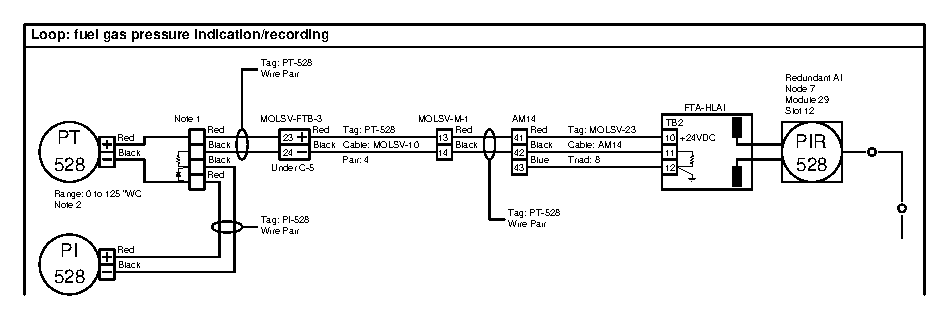
\includegraphics[width=15.5cm]{i00112x04.eps}$$








\vfil \eject

\noindent
{\bf Lab questions}

\vskip 20pt

\item{$(1)$} Sketch connecting wires necessary to make this loop-powered DP transmitter provide a signal to the controller's analog input \#1:

$$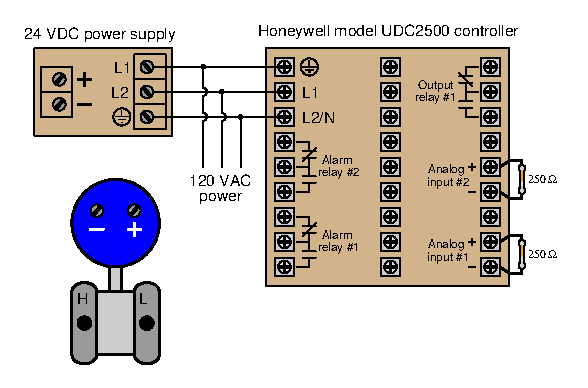
\includegraphics[width=15.5cm]{i00112x06.eps}$$

\vskip 20pt

\item{$(2)$} Identify and explain {\it maximum working pressure} (MWP, also known as ``maximum static pressure'') of your pressure transmitter, especially how it differs from the {\it maximum calibrated range} (LSL and USL) of the transmitter.

\vskip 20pt

\item{$(3)$} Calculate the allowable pressure error for a pressure transmitter given a range of 0 to 250 PSI and an allowable percentage of span error of $\pm$ 0.5\%.

\vskip 20pt

\item{$(4)$} PIR-528 shows a value of 133 "WC (``pegged'' high) for its process variable (PV) display.  An instrument technician measures 0 VDC between terminals 13 and 14.  Identify \underbar{two} different faults which could account for these symptoms, being as specific as possible in your answers:

$$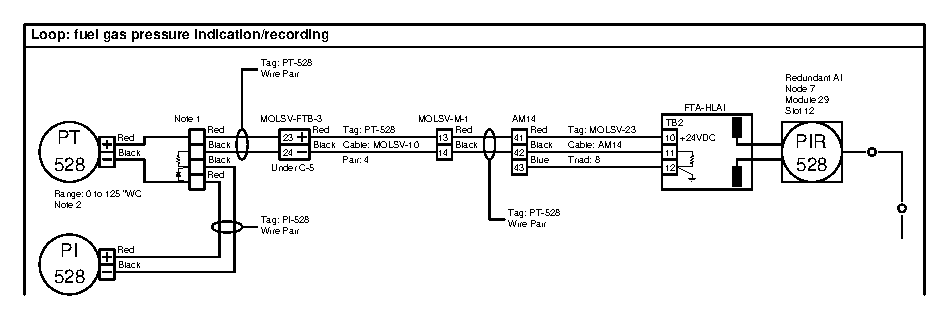
\includegraphics[width=15.5cm]{i00112x04.eps}$$


%INDEX% Lab exercise, deadweight tester
%INDEX% Lab exercise, electronic DP transmitter
%INDEX% Lab exercise, pressure measurement loop

%(END_NOTES)


